\section{Performance Evaluation of Nonlinear Solution Convergence}
%

\begin{figure}[!tbhp]
\centering
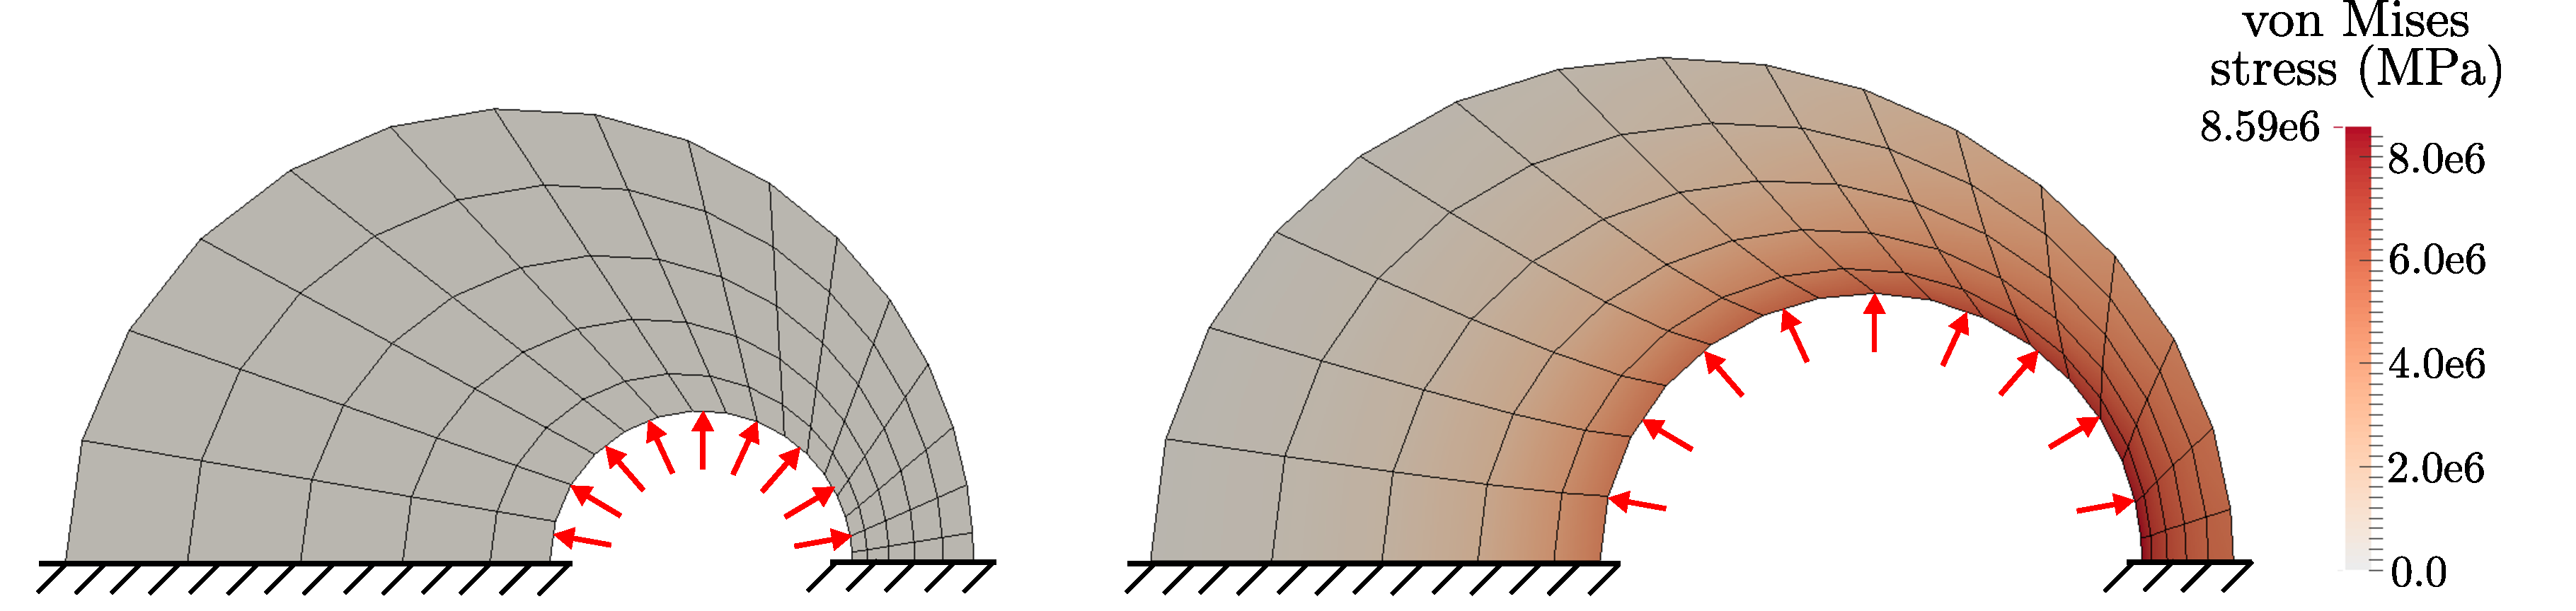
\includegraphics[scale=0.28]{media/ring_problem}
% where an .eps filename suffix will be assumed under latex,
% and a .pdf suffix will be assumed for pdflatex
\caption{Pressurized eccentric cylinder modeled with half-symmetry.}
\label{fig.ring}
\end{figure}

\begin{table}[]
\centering
\caption{Number of Newton-Raphson iterations per time step for the eccentric cylinder problem}
\label{tab.ring}
\begin{tabular}{|c|c|c|c|}
\hline
Step & Hughes-Winget & Rashid (1993) & Proposed Algorithm  \\ \hline
1  & 3 & 3  & 3 \\ \hline
2  & 2 & 2  & 2 \\ \hline
3  & 2 & 2  & 2 \\ \hline
4  & 2 & 2  & 2 \\ \hline
5  & 2 & 2  & 2 \\ \hline
6  & 2 & 3  & 2 \\ \hline
7  & 2 & 3  & 2 \\ \hline
8  & 2 & 3  & 2 \\ \hline
9  & 3 & 4  & 3 \\ \hline
10 & 4 & 27 & 4\\ \hline
\end{tabular}
\end{table}

\begin{table}[]
\centering
\caption{Number of Newton-Raphson iterations using an inconsistent linearization}
\label{tab.ring_tangents}
\begin{tabular}{|c|c|c|c|c|}
\hline
Step & Consistent & Rotation Off & Pressure Off & Rotation \& Pressure Off \\ \hline
1  & 3 & 5   & 6  & 6 \\ \hline
2  & 2 & 5   & 7  & 8 \\ \hline
3  & 2 & 6   & 9  & 10 \\ \hline
4  & 2 & 6   & 11 & 13 \\ \hline
5  & 2 & 8   & 14 & 16 \\ \hline
6  & 2 & 10  & 18 & 20 \\ \hline
7  & 2 & 14  & 25 & 24 \\ \hline
8  & 2 & 22  & 42 & 31 \\ \hline
9  & 3 & 40  & 123 & 41 \\ \hline
10 & 4 & 771 & $>$1000 & 784 \\ \hline
\end{tabular}
\end{table}